\documentclass[ms,electronic,letterpaper,lol,lof]{byumsphd}

\usepackage{amsmath}
\usepackage{graphicx}
\usepackage{listings}
%\usepackage[outputdir=build]{minted}
\usepackage{inconsolata}
\usepackage[T1]{fontenc}
\usepackage{natbib}
\usepackage{tikz}
\usetikzlibrary{positioning}
\usepackage{amsthm}

\newcommand{\racket}[1]{\mintinline{racket}{#1}}
% TODO: use natbib maybe?
\begin{document}

\title{Enabling Optimizations through Demodularization} 

\author{Blake Johnson}

\committeechair{Eric Mercer}
\committeemembera{Christophe Giraud-Carrier}
\committeememberb{Quinn Snell}

\monthgraduated{December}
\yeargraduated{2015}
\yearcopyrighted{2015}

\documentabstract{%
Programmers want to write modular programs to increase maintainability and create abstractions, but modularity hampers optimizations, especially when modules are compiled separately or written in different languages. 
In languages with syntactic extension capabilities, each module in a program can be written in a separate language, and the module system must ensure that the modules interoperate correctly. 
In Racket, the module system ensures this by separating module code into phases for runtime and compile-time and allowing phased imports and exports inside modules. 
We present an algorithm, called demodularization, that combines all executable code from a phased modular program into a single module that can then be optimized as a whole program. 
The demodularized programs have the same behavior as their modular counterparts but are easier to optimize. 
We show that programs maintain their meaning through an operational semantics of the demodularization process and verify that performance increases by running the algorithm and existing optimizations on Racket programs.
}


\documentkeywords{macros, Racket, modules, optimization}

\acknowledgments{Jay McCarthy, Matthew Flatt, Eric Mercer}

\department{Computer~Science}
\graduatecoordinator{Quinn~Snell}
\collegedean{Thomas~W.~Sederberg}
\collegedeantitle{Associate~Dean}
\maketitle

\chapter{Introduction}

Programmers should not have to sacrifice the software engineering goals of modular design and good abstractions for performance. 
Instead, their tools should make running a well-designed program as efficient as possible. 

Many languages provide features for creating modular programs which enable separate compilation and module reuse.
Some languages provide expressive macro systems, which enable programmers to extend the compiler in arbitrary ways.
Combining module systems with expressive macro systems allow programmers to write modular programs with each module written in its own domain-specific language.
A compiler for such a language must ensure that modular programs have the same meaning independent of the order in which the modules are compiled.
A phased module system, like the one described by Flatt \cite{Flatt} for Racket, is a way to allow both separately compiled modules and expressive macros in a language.

Modular programs are difficult to optimize because the compiler has little to no information about values that come from other modules when compiling a single module.
Existing optimizations have even less information when modules can extend the compiler. 
Good abstractions are meant to obscure internal implementations so that it is easier for programmers to reason about their programs, but this obscurity also limits information available for optimizations.  
In contrast, non-modular programs are simpler to optimize because the compiler has information about every value in the program.

Some languages avoid the problem of optimizing modular programs by not allowing modules, while others do optimizations at link time, and others use inlining. 
Not allowing modules defeats the benefits of modular design. 
Link time optimizations can be too low level to do useful optimizations. 
Inlining must be heuristic-based, and good heuristics are hard to develop. 

Our solution for optimizing modular programs, called demodularization, is to transform a modular program into a non-modular program by combining all runtime code and data in the program into a single module.
In a phased module system, finding all of the runtime values is not trivial.
Phased module systems allow programmers to refer to the same module while writing compiler extensions and while writing normal programs.
A demodularized program does not need to include modules that are only needed during compile-time, but whether or not the module is needed only at compile-time is not obvious from just examining the module in isolation. 

A program with a single module is effectively a non-modular program. After demodularization, a program becomes a single module, so existing optimizers have more information. Also, demodularization enables new optimizations that need whole program information. 

We provide an operational semantics for a simple language with a phased module system, and argue that the demodularization process preserves program meaning. We also provide an implementation of demodularization for the Racket programming language, and verify experimentally that programs perform better after demodularization.

% TODO make the chapter references into actual refs
We explain demodularization at a high level with a detailed example (Chapter 2). Next, we use the operational semantics model of the demodularization process to explain why demodularization is correct (Chapter 3), then describe an actual implementation for Racket (Chapter 4), followed by experimental results of demodularizing and optimizing real-world Racket programs (Chapter 5). The operational semantics model removes the unnecessary details of the full implementation so the demodularization process is easier to understand and verify. The actual implementation presents interesting difficulties that the model does not. The experimental results show that demodularization improves performance, especially when a program is highly modular. 

\chapter{The Racket Module System}
\label{chap:module-system}

% DONE: rewrite this section
\section{The Racket Programming Language}
The Racket Programming Language is a platform for creating powerful abstractions.
These abstractions are created through the use of Racket's macro and module systems. 
The macro system, a heritage from LISP~\cite{} and Scheme~\cite{}, allows programmers to add new features to their programs in an integrated way.
The module system allows programmers to separate their programs into logical parts and hide implementation details. 
Together, they allow programmers to create Languages as Libraries~\cite{} that are suitable for specific tasks.

% TODO: mention that programs can extend themselves in the same file
\section{Macros}
Macros are the main way programmers add new features to Racket. 
Esentially, macros are functions (known as transformers) whose domain and range are syntax objects.
Syntax objects are data structures that contain the raw syntax of a program, along with lexical information and other properties associated with the syntax.
If a programmer needs the power, they can write transformers using all of the features of Racket, as long as the function takes in and produces syntax objects.
Racket provides pattern-matching for syntax objects that makes writing macros simpler when that is all that a programmer needs.

The \racket{define-syntax} form is used to identify a macro definition that is a funtion from syntax to syntax.
The helper function, \racket{syntax-case} matches syntax patterns so that it is easy to use them in the output of the macro.

% DONE: example should use a function or letrec, not let loop
% DONE: maybe just use syntax-case here
\begin{listing}
  \inputminted{racket}{listings/while-macro.rkt}
  \caption{a macro implementation of a \racket{while} loop}
  \label{lst:while-macro.rkt}
\end{listing}
Listing~\ref{lst:while-macro.rkt} shows how to use one of these macros to write a \racket{while} loop. 
The macro turns a \racket{while} loop into a recursive function and a call to that recursive function.
Whatever syntax used by the programmer for the \racket{test} and \racket{body ...} forms will be substituted into the output of the macro. 
Listing~\ref{lst:while-expanded.rkt} shows a use of the while macro and what it expands into after running the macro. 
\begin{listing}
  \inputminted{racket}{listings/while-expanded.rkt}
  \caption{use and expansion of a \racket{while} loop}
  \label{lst:while-expanded.rkt}
\end{listing}
% DONE: example expansion
% DONE: fuller explanation of hygeine with citation
Racket's macros are hygenic \cite{}, which means that identifiers created from programs will not clash with identifiers created from macros. 
In this example that means that the Racket program using a while loop will not be able to call the \racket{while-loop} function that the macro creates, and that if the program has another definition for \racket{while-loop}, it will be independent from the definition introduced by the macro.
Also, each use of the macro will have distinct definitions for \racket{while-loop} so that the macro can be nested and used multiple times.
\section{Modules}
% TODO: all listings are modules in separate files
Racket modules are a way of grouping definitions, expressions, and macros into groups. 
Modules also allow control over imports and exports, using the Racket forms \racket{require} and \racket{provide} respectively.
Listing~\ref{lst:counter.rkt} shows a simple Racket module and some of the features of the Racket module system.
\begin{listing}
  \inputminted{racket}{listings/counter.rkt}
  \caption{\texttt{counter.rkt}: A simple Racket module implementing a counter}
  \label{lst:counter.rkt}
\end{listing}
The \texttt{counter} module contains a variable definition and functions for getting and incrementing that variable.
The module only exports the functions, so the module encapsulates the variable.
If a programmer wanted to use this module, they would import it using \racket{require} as shown in Listing~\ref{lst:while-test.rkt}. 

\begin{listing}
  \inputminted{racket}{listings/while-test.rkt}
  \caption{\texttt{while-test.rkt}: A Racket module that uses other modules}
  \label{lst:while-test.rkt}
\end{listing}

It is also possible to use modules to help write macros.
For example, if a programmer wanted to change the \racket{while} macro so that it reported how many expressions were in each while loop, they could use the \texttt{counter} module inside the \racket{while} definition as seen in Listing~\ref{lst:while-lang.rkt}.
\begin{listing}
  \inputminted{racket}{listings/while-lang.rkt}
  \caption{\texttt{while-lang.rkt}: A Racket module implementing a language with \racket{while} loops}
  \label{lst:while-lang.rkt}
\end{listing}
It is possible to add code to the \racket{while} macro because it is just a function from syntax to syntax that runs at compile-time. 
Also, the \racket{require} form includes a \racket{for-syntax} form to indicate that the \texttt{counter} module is needed at compile-time (along with the \racket{racket/base} module for \racket{printf}).
Now this module can be used to extend the language of other programs by adding a \racket{while} loop, but it is just a library that is included like any other library.

\section{Languages}
% TODO: Rewrite this section, it sucks
The ability to use modules as languages allows programmers to write specialized domain-specific languages (DSLs) to better express solutions to domain problems. 
% TODO: akward sentence
Using this ability, programmers have added languages for Typed Racket~\cite{}, Object-Oriented Racket~\cite{}, Logic Programming~\cite{}, and more~\cite{}.
Also, because they are modules, it is possible to use them all in the same program and use the right language for each specific problem.
The language creating facilities of Racket extend to more than just collections of functions and macros; they also allow changing the parser and changing the meaning of things like function application syntax. 

\section{Separate Compiliation}
In the presence of macros that can run arbitrary code, compilation of a single module becomes complicated. 
Compilation and execution of code has to be interleaved in order to produce the correct compiled program.
% DONE: explain that listings form a program with multiple modules and while-test is main
% DONE: include module dependency figure
All of the listings in the previous section form a program with the \racket{while-test} module as the main module.
Figure~\ref{fig:modules.tex} shows the relationship between the different modules in the program.
\begin{figure}
  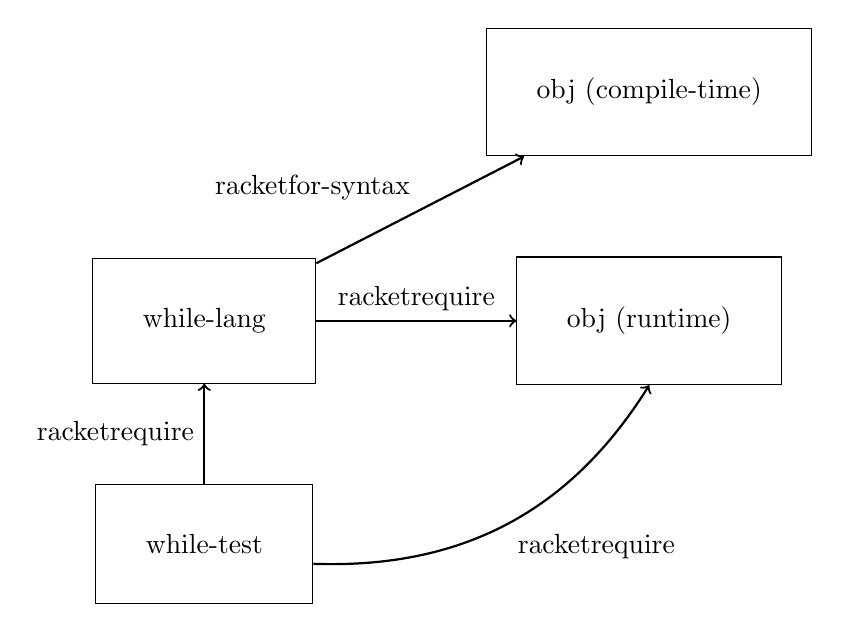
\begin{tikzpicture}
  [node distance=.5in and 1in,
   module/.style={rectangle,draw,inner sep=.25in}
  ]
\node (obj-comp)   [module] {obj (compile-time)};
\node (obj-run)    [module] [below=of obj-comp] {obj (runtime)};
\node (while-lang) [module] [left=of obj-run] {while-lang}
  edge [->, thick] node[auto]{\racket{require}} (obj-run)
  edge [->, thick] node[auto]{\racket{for-syntax}} (obj-comp);
\node (while-test) [module] [below=of while-lang] {while-test}
  edge [->, thick] node[auto]{\racket{require}} (while-lang) 
  edge [->, thick, bend right] node[swap,auto]{\racket{require}} (obj-run.south);
\end{tikzpicture}

  \caption{Module dependencies for the \racket{while-test} program}
  \label{fig:modules.tex}
\end{figure}
To compile the program, both the \racket{while-lang} and \racket{counter} need to be compiled before \racket{while-test}, but also the \racket{counter} module needs to be compiled and ready to use while compiling \racket{while-test} because the counter functions are used inside the \racket{while} macro.
While compiling \racket{while-test}, the \racket{while} macro will be expanded and code from the \racket{counter} module will run.
The value of the counter is not shared between compiling \racket{while-test} and running it.

\section{Phases}
The way the Racket module system allows for reliable separate compiliation is by separating compilation and execution into phases.
Phase 0 is the execution phase of the main module of a program, what could be considered running the program.
Phase 1 is the compilation phase of the main module, which could include execution of code inside macros. 
Phase 2 is the compiliation phase of any modules that need to execute during phase 1, and higher phases are used as needed to compile and run code used in lower phases.
% TODO: awkward sentence
% TODO: maybe explain for-template better (first time introduced)
It is possible for modules to reference modules at higher phases by using the \racket{for-syntax} form as seen above, and it is also possible to reference modules at lower phases by using the \racket{for-template} form.

In the example above, the \racket{while-test} module is compiled at phase 1, which triggers compilation of the \racket{counter} module at phase 2, so that the \racket{counter} module can be instantiated at phase 1 to count how many expressions are in the \racket{while} loop.
The phase 1 instantiation of the \racket{counter} module is separate from the phase 0 instantiation of the module.
This is a guarantee of the Racket module system, that ``Any effects of the instantiation of the module's phase 1 due to compilation on the Racket runtime system are discarded,'' which is known as the "Separate Compilation Guarantee"~\cite{}.

\section{Program Evaluation}
Running a separately compiled Racket program involves following all of the \racket{require} forms and running all phase 0 code in the order they were imported.
It is possible that phase 0 code will come through a module that is required by using \racket{for-syntax} if somewhere along the line code is then required using \racket{for-template}.

By understanding how Racket programs are compiled and evaluated, it is apparent that only phase 0 code is necessary to run the program. 
This is the basis for how demodularization can recover whole programs from separately compiled Racket modules. 

\chapter{Intuition}
\label{chap:intuition}
Demodularization is the process of collecting all phase 0 code required by a program into a single module.
This is done by tracing through the \racket{require} graph starting at a program's main module.
The following example program illustrates the need for demodularization and how it is done.

\section{Example Program}
A programmer wants to use a queue library where the library uses different backing structures depending on the length of the queue. 
Listing~\ref{lst:main.rkt} shows an example of using such a library.
\begin{listing}
  \inputminted{racket}{listings/main.rkt}
  \caption{\texttt{main.rkt} module with queue usage}
  \label{lst:main.rkt}
\end{listing}
The library is implemented as a macro, show in Listing~\ref{lst:queue.rkt}, that switches between two implementatations depending on the length of the initial queue.
\begin{listing}
  \inputminted{racket}{listings/queue.rkt}
  \caption{\texttt{queue.rkt} module}
  \label{lst:queue.rkt}
\end{listing}
Listing~\ref{lst:long-queue.rkt} and Listing~\ref{lst:short-queue.rkt} show the two queue implementations, with the \texttt{long-queue} using vectors and the \texttt{short-queue} using lists. 
% DONE: say that ... is actual racket syntax
The \racket{....} signifies elided code (but \racket{...} has meaning in Racket).

\begin{listing}
  \inputminted{racket}{listings/long-queue.rkt}
  \caption{\texttt{long-queue.rkt} module}
  \label{lst:long-queue.rkt}
\end{listing}

\begin{listing}
  \inputminted{racket}{listings/short-queue.rkt}
  \caption{\texttt{short-queue.rkt} module}
  \label{lst:short-queue.rkt}
\end{listing}


\section{Compilation}

Compiling this program involves expanding the \racket{with-queue} macro, which will turn the program into Listing~\ref{lst:main-expanded.rkt}.

\begin{listing}
  \inputminted{racket}{listings/main-expanded.rkt}
  \caption{\texttt{main.rkt} module after macro expansion}
  \label{lst:main-expanded.rkt}
\end{listing}

The expanded program contains references to \racket{long-queue} operations because the length of the initial queue was over 5.
While the expanded program is not the same as a fully compiled program, it can stand in for one with regard to optimization and demodularization.

With the expanded program, it is possible to see how cross-module optimizations would be difficult.
The program has calls to functions in the \racket{long-queue} module, so the optimizer does not have access to the definitions of the functions while finishing the compilation of the main module.

\section{Demodularization}

Demodularization of the program proceeds by following the \racket{require} graph and including phase 0 code. 
The \racket{main} module requires the \racket{queue} module, but the \racket{queue} module only has phase 1 code, so it is not included in the final module.
The \racket{queue} module requires the \racket{long-queue} and \racket{short-queue} modules, which have various phase 0 definitions that get included in the order they appear in their original modules.
Listing~\ref{lst:main-demodularized.rkt} shows what the demodularized example program would look like.

\begin{listing}
  \inputminted{racket}{listings/main-demodularized.rkt}
  \caption{\texttt{main.rkt} module after demodularization}
  \label{lst:main-demodularized.rkt}
\end{listing}

% DONE: make a point that extra queue implementation is there
The demodularized program should have the exact same behavior at runtime as the modular program.
At this point, the only thing that changes is that the Racket runtime does not need to follow the \racket{require} graph because all phase 0 definitions and expressions are in a single module.
Also, both queue implementations appear in the demodularized program even though only one of them is used.


\section{Optimization}

After a program has been demodularized, the optimizer now has all the information it needs to do optimizations on the whole program.
Listing~\ref{lst:main-optimized.rkt} shows what the example program would look like after optimization.

\begin{listing}
  \inputminted{racket}{listings/main-optimized.rkt}
  \caption{\texttt{main.rkt} module after optimization}
  \label{lst:main-optimized.rkt}
\end{listing}

% DONE: point out that the dead code is eliminated
The optimizer is able to inline the various functions because it has access to all of the definitions within the module.
The optimizer also removes the extra queue implementation because it is dead code.
Therefore, demodularization enables optimization by providing the optimizer access to the whole program in one place.

\chapter{Model}
\label{chap:model}

We can understand the specifics of demodularization by describing it as an algorithm for a simple language with a well defined semantics.

\section{A Module Language}
The \emph{mod} language (Figure~\ref{fig:source-lang}) contains only the features necessary to write modular programs where it is possible to observe the effects of module evaluation order.

\begin{figure}[h]
\centering
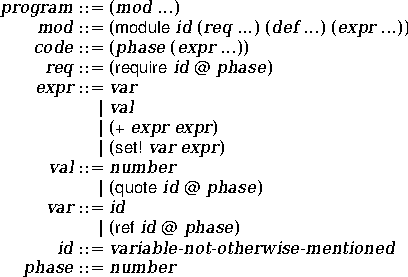
\includegraphics{figures/source}
\caption{\emph{mod} language grammar}
\label{fig:source-lang}
\end{figure}

A program in \emph{mod} consists of a list of modules that can refer to each other.
Each module has a name, any number of imports, any number of definitions, and sequenced code expressions. 
All definitions in a module are exposed as exports to other modules, but to use definitions from another module, the program must import it through a \racket{require} expression.
Both \racket{require} and \racket{define} expressions have phase annotations; this simulates the interactions between modules in a language with macros and a language tower without requiring a model of macro expansion.
The language includes variable references, numbers, addition, and mutation.
Mutation makes module evaluation order observable, and addition represents the work that a module does.
In addition to numbers and variables, there are two special forms of values and references that model the interaction of macros with the module system.
A \racket{quote} expression is like a reference to syntax at runtime.
A \racket{ref} expression is like a macro that can only do one thing: refer to a variable at a phase.

\section{Compilation}

We have to compile \emph{mod} programs before demodularizing them, just like in the Racket implementation.
In Racket, compiling expands all macros in a program and changes definitions and variable references to refer to memory locations.
In \emph{mod}, compiling eliminates \racket{ref} expressions, turns definitions into \racket{set!} expressions, changes variable references to include module information, and sorts code into phases.
Compilation in both cases still leaves behind a relatively high-level language, but the language is free of syntactic extensions.
This is important for demodularization because otherwise macro expansion would have to be part of the algorithm, which would complicate it and possibly duplicate work.
The grammar in Figure~\ref{fig:compiled-lang} specifies the compiled language for \emph{mod}.

\begin{figure}[h]
\centering
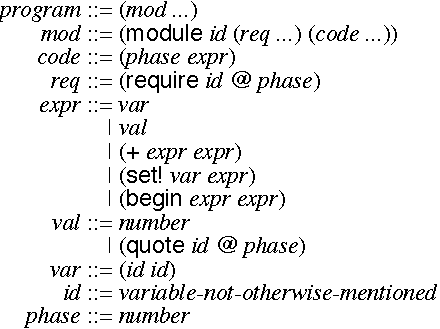
\includegraphics{figures/compiled-lang}
\caption{Compiled language grammar}
\label{fig:compiled-lang}
\end{figure}

The grammar no longer has definitions, all variables now include module references, and code is sorted into phases.
The actual compilation function is not relevant to demodularization.

\section{Evaluation}

We evaluate the compiled language using a small-step reduction semantics. 
Because the reduction rules are syntactic, we extend the compiled language further with evaluation contexts, a heap representation, and a stack representation to keep track of the order to instantiate modules.
These extensions are in Figure~\ref{fig:compiled-eval-lang}.
An expression of the form:
\[
  (\sigma\ /\ program\ /\ ((id\ phase)\ \ldots)\ /\ ((id\ phase)\ \ldots))
\]
represents the state of the machine during evaluation.
$\sigma$ represents the heap of the program, and when evaluation finishes represents the output of the program.
The list of modules is the code of program in the compiled language.
The first list of \emph{(id phase)} pairs is the list of modules to evaluate, and the second list is the modules that have already been evaluated.

\begin{figure}[h]
\centering
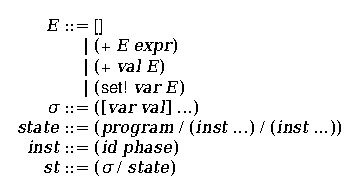
\includegraphics{figures/compiled-eval-lang}
\caption{Extensions to compiled language grammar}
\label{fig:compiled-eval-lang}
\end{figure}

The reduction rules in Figures~\ref{fig:eval-reduction0}--\ref{fig:eval-reduction6} evaluate a compiled program that starts with an empty heap, the program code, a stack that contains the identifier of the main module at phase 0, and an empty completed module list. 

% DONE: re-render without red
% DONE: maybe needs a rewrite to capture meaning better (Jay's example)
\begin{figure}[!h]
  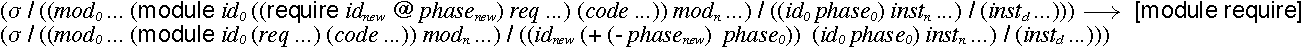
\includegraphics[width=\textwidth]{figures/eval-reduction0}
\caption{\emph{module require} rule for modular evaluation}
\label{fig:eval-reduction0}
\end{figure}
% TODO: explain that phases are relative
The \emph{module require} rule in Figure~\ref{fig:eval-reduction0} matches a program with a \racket{require} expression in the module at the top of the evaluation stack and evaluates it by removing the \racket{require} expression from the module and pushing the required module onto the evaluation stack with the phase shifted appropriately.
The current module is still on the stack and will continue evaluating after the required module is done evaluating.
The subsequent rules all apply only when the phase relative to the main module is zero.

\begin{figure}[!h]
  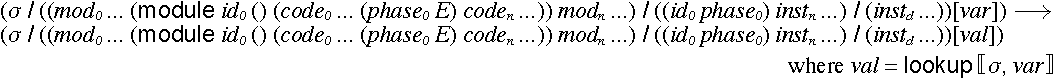
\includegraphics[width=\textwidth]{figures/eval-reduction1}
\caption{\emph{var ref} rule for modular evaluation}
\label{fig:eval-reduction1}
\end{figure}
The \emph{var ref} rule in Figure~\ref{fig:eval-reduction1} looks up a variable in the heap and replaces the variable with its current value.
The lookup function is a simple list lookup function that matches the variable name with its occurence in the heap. 

\begin{figure}[!h]
  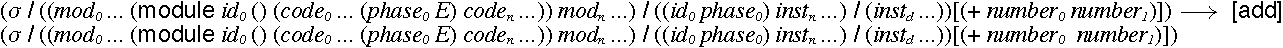
\includegraphics[width=\textwidth]{figures/eval-reduction2}
\caption{\emph{add} rule for modular evaluation}
\label{fig:eval-reduction2}
\end{figure}
The \emph{add} rule in Figure~\ref{fig:eval-reduction2} replaces an addition expression of numbers with the result of computing their sum.
The rule uses the standard Racket implementation of plus to compute the sum.

\begin{figure}[!h]
  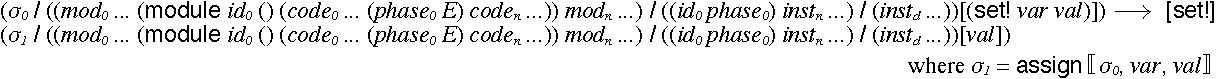
\includegraphics[width=\textwidth]{figures/eval-reduction3}
\caption{\emph{set!} rule for modular evaluation}
\label{fig:eval-reduction3}
\end{figure}
The \emph{set!} rule in Figure~\ref{fig:eval-reduction3} installs a value for a variable into the heap and reduces to the value.
The assign function either replaces the existing value for a variable in the heap or installs a new entry in the heap if it does not exist already.

\begin{figure}[!h]
  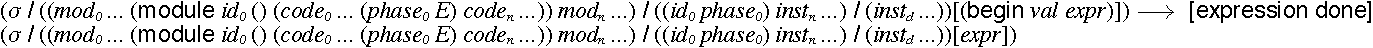
\includegraphics[width=\textwidth]{figures/eval-reduction4}
\caption{\emph{expression done} rule for modular evaluation}
\label{fig:eval-reduction4}
\end{figure}
When an expression is a value, the \emph{expression done} rule in Figure~\ref{fig:eval-reduction4} matches and removes the expression from the module.

\begin{figure}[!h]
  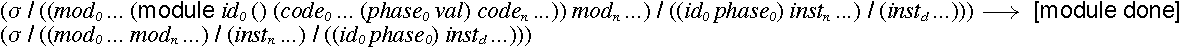
\includegraphics[width=\textwidth]{figures/eval-reduction5}
\caption{\emph{module done} rule for modular evaluation}
\label{fig:eval-reduction5}
\end{figure}
When there are no more expressions left in a module, the \emph{module done} rule in Figure~\ref{fig:eval-reduction5} applies by removing the module from the program and placing a reference to it in the list of finished modules.

\begin{figure}[!h]
  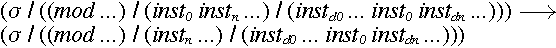
\includegraphics{figures/eval-reduction6}
\caption{\emph{module done already} rule for modular evaluation}
\label{fig:eval-reduction6}
\end{figure}
The \emph{module done already} rule in Figure~\ref{fig:eval-reduction6} applies when the current module on the stack is in the finished list, so that modules are not evaluated multiple times. 

\section{Demodularization}

Figures~\ref{fig:demod-redex0}--\ref{fig:demod-redex3} shows the demodularization algorithm for the compiled language.
The algorithm takes as input an \emph{id} specifying the main module of the program, a working list of phased requires, and a list of modules that make up the program.


\begin{figure}[!h]
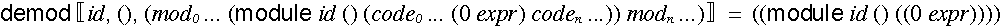
\includegraphics[width=\textwidth]{figures/demod-redex0}
\caption{Demodularization algorithm}
\label{fig:demod-redex0}
\end{figure}
The first rule in Figure~\ref{fig:demod-redex0} applies when the main module has no requires left and there are no requires in the working list, meaning the algorithm can terminate with just the phase 0 code of the main module remaining.
\begin{figure}[!h]
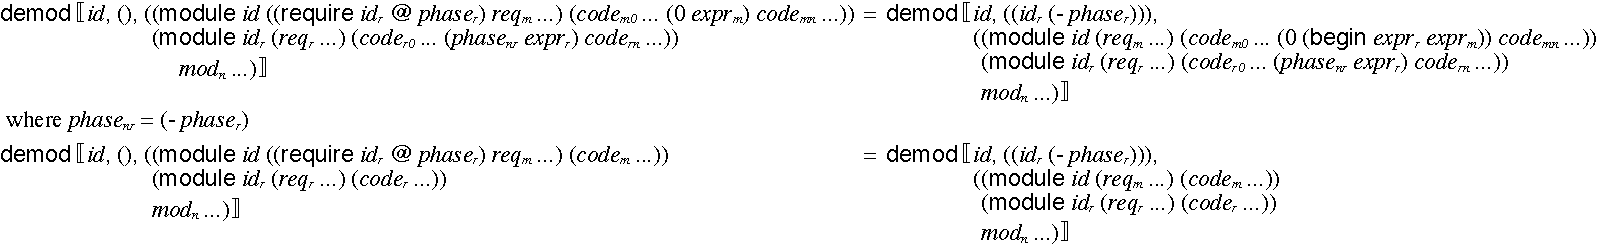
\includegraphics[width=\textwidth]{figures/demod-redex1}
\caption{Demodularization algorithm}
\label{fig:demod-redex1}
\end{figure}
The second and third rules in Figure~\ref{fig:demod-redex1} apply when the main module requires the next module in the module list.
Both rules add the required module's \emph{id} to the working list of required modules so that the algorithm will follow the complete require graph.
% TODO: check to see if there is a diamond pattern, will the algorithm handle it correctly (I don't think it will right now)
The second rule handles the case where the required module has code that will be at phase 0 for the main module and puts that code before the existing phase 0 code of the main module.
\begin{figure}[!h]
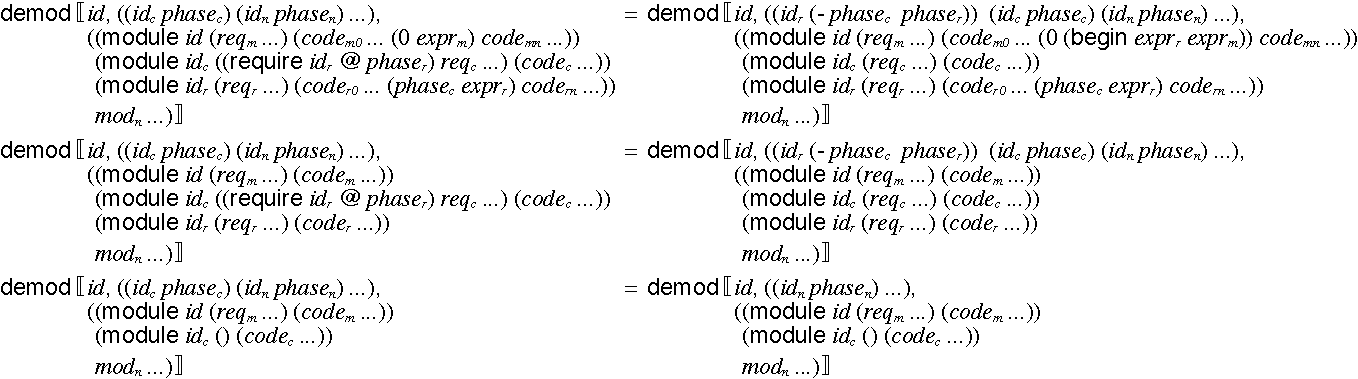
\includegraphics[width=\textwidth]{figures/demod-redex2}
\caption{Demodularization algorithm}
\label{fig:demod-redex2}
\end{figure}
The next three rules in Figure~\ref{fig:demod-redex2} apply when handling the working list of required modules. 
The first of the three is similar to the second rule because it extracts code that will be in phase 0 of the main module and inserts it into the main module.
The second rule of the three working list rules handles the case where there is no matching code for phase 0.
The third rule removes an entry from the working list when the module has no more requires.

\begin{figure}[!h]
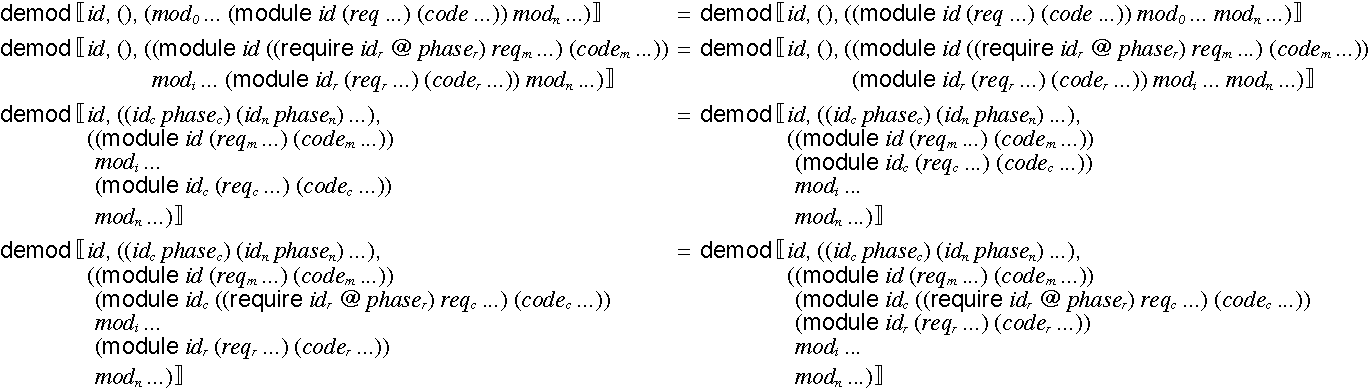
\includegraphics[width=\textwidth]{figures/demod-redex3}
\caption{Demodularization algorithm}
\label{fig:demod-redex3}
\end{figure}

The final four rules in Figure~\ref{fig:demod-redex3} rearrange the program's module list so that modules that require each other are adjacent in the list and the other rules can apply.

\section{Equivalence}
We claim that the programs will evaluate to the same answers before and after demodularization. 

\newtheorem*{theorem}{Theorem}
\begin{theorem}
Evaluating a program P a number of steps n and the demodularized program $P'$ a number of steps m will be bisimilar with respect to the stores of the programs as shown in Figure~\ref{fig:bisim.tex}.
\end{theorem}

\begin{figure}[h]
  \centering
  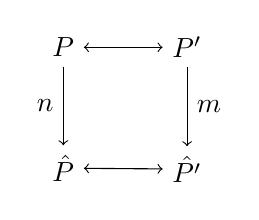
\begin{tikzpicture}
\node (P) at (0,0) {$P$};
\node [right=of P] (P') {$P'$};
\node [below=of P] (Phat) {$\hat{P}$};
\node [below=of P'] (P'hat) {$\hat{P'}$};
\draw[<->] (P)--(P');
\draw[<->] (Phat)--(P'hat);
\draw[->]  (P)--(Phat) node [midway,left] {$n$};
\draw[->]  (P')--(P'hat) node [midway,right] {$m$};
\end{tikzpicture}

  \caption{Bisimulation of a program before and after demodularization}
  \label{fig:bisim.tex}
\end{figure}

\begin{proof}
The proof is by induction on the DAG of required modules in a program.
For each shape of possible requires in a program, we would show the evaluation before and after demodularization end up running the same module code in the same order and result in the same stores.
\end{proof}

The full proof of the theorem would not be instructive because of the complexities of the implementation of the model and the demodularization algorithm.


\chapter{Implementation}
\label{chap:implementation}

The implementation of demodularization for the Racket module system is included in the Racket distribution as part of the build tool \racket{raco}. 
Users can pass in a module they would like to demodularize and optmize to the tool and it will compile all the necessary modules, run the demodularization algorithm on them, decompile the resulting module, and run optimizations on it to produce the final module.
The demodularization algorithm runs on compiled modules, which are stored in Racket bytecode files.

\section{Racket bytecode}
Racket bytecode is different from most other forms of bytecode in that it mostly maintains the structure of the abstract syntax tree from the original program.
The main aspect that changes between fully-expanded Racket programs and Racket bytecode is the use of stack positions instead of variables and the addition of stack-manipulating instructions.
A full explanation of Racket bytecode and what it means can be found in \ref{}.

% DONE: Don't start a paragraph with Also
A table is created in the bytecode for the top level bindings in a module, which is known as the prefix.
All top level bindings have an entry in the prefix, including bindings that come from other modules, and any use of a top level binding in a program is replaced with a numeric reference to the entry.
Listing~\ref{lst:kernel.rkt} shows a simple program written in the most basic language that Racket supports: the \racket{kernel} language.
\begin{listing}
  \inputminted{racket}{listings/kernel.rkt}
  \caption{Example program written in \racket{kernel} language}
  \label{lst:kernel.rkt}
\end{listing}
When this code is compiled, it turns into the bytecode in Listing~\ref{kernel-bytecode.rkt}. 
\begin{listing}
  \inputminted{racket}{listings/kernel-bytecode.rkt}
  \caption{Bytecode representation of program from Listing~\ref{lst:kernel.rkt}}
  \label{lst:kernel-bytecode.rkt}
\end{listing}

% DONE: comment on primval
In the bytecode, all references to the variable \racket{y} have been replaced with references to the prefix in the form of \racket{(toplevel 0)}. 
All references to \racket{displayln} have also been replaced with \racket{(toplevel 1)} references, which in turn references element \racket{7} of the prefix of the \racket{racket/private/misc} module.
The references to \racket{x} are now all different because the stack changes between each usage of \racket{x}.
The references to \racket{random} and \racket{+} are replaced with references to primitive implementations in the Racket runtime. 

\section{Demodularization}

The implementation of demodularization for the Racket module system is written in Racket and consumes and produces Racket bytecode.
The library for reading and writing Racket bytecode in Racket was mainly used for debugging purposes and was incomplete, so the first task was to fully implement the Racket bytecode library.

The actual algorithm for demodularization is similar to the model in the previous chapter in that it traces requires and includes all phase 0 code in the final module, but it also has to deal with the module prefix and references to the prefix.
When the algorithm includes a required module, it also includes that module's prefix appended to the end of the main module's prefix. 
Then, it must adjust all references in that module's code to point at the new combined prefix.
Also, the algorithm tracks cross-module references and rewrites them to point to the new prefix as well.
In the example in Listing~\ref{lst:kernel-bytecode.rkt}, when the algorithm includes the module \racket{racket/private/misc} it must rewrite the reference to \racket{(toplevel 1)} to whatever the new position for \racket{displayln} is in the combined prefix.
% TODO: show a demod example

\section{Optimization}

For demodularization to be useful, the program needs to be optimized after demodularizing it.
% TODO: relate back to thesis rather than say we wanted
To optmize the demodularized bytecode, we wanted the existing Racket optimizer built into the Racket compiler so that we get all existing optimizations ``for free'' and any new optimizations in the future will work on both regularly compiled and demodularized programs.
The existing optimizer works on an intermediate form between fully-expanded Racket code and Racket bytecode.
This intermediate form only exists as C data structures in the implementation of Racket.
Therefore, to use the existing optimizer, Racket bytecode needed to be decompiled into this intermediate form. 

\section{Decompilation}

The decompiler was written in C, so that it could interoperate with the optimizer.
There are three main differences between Racket bytecode and the intermediate form: stack positions, cyclic closures, and reference arguments.
In Racket bytecode and in the intermediate form, all references to bindings are numeric, but in bytecode the references are stack positions and in the intermediate form the references are lexical.
For example, the bytecode in Listing~\ref{lst:kernel-bytecode} has three references to \racket{x}, in the form of \racket{(install-value 0 5)}, \racket{(local 1)}, and \racket{(local 3)}. 
% DONE: explain why they should all be 0
In the intermediate form, all of these references to \racket{x} should be \racket{0} because lexically they all refer to the same variable that is the closest binding.

Racket bytecode allows for cyclic closures, or closures which contain a reference to themselves.
Nothing like this exists in the intermediate form, so to decompile cyclic closures, the decompiler creates a new top level definition for the closure and replaces references to the closure (including the self-references) with references to the top level definition.
% TODO: maybe an example of this as well

Finally, Racket bytecode allows reference arguments (like C++ reference arguments) in functions, but the intermediate form doesn't allow them.
The decompiler turns reference arguments into \racket{case-lamdba} closures over the reference arguments with one case for getting the argument value and one case for setting the argument value. 

% TODO: how to know if it works (verification) paragraph
The decompilation algorithm is not the identity function when composed with compilation because of the transformations performed on cyclic closures and reference arguments.
Sometimes the optimizer will remove the \racket{case-lambda} arguments and turn them back into reference arguments, but this is not guaranteed. 
Racket has robust bytecode verification built in to the module loading system, so errors that were introduced by the decompiler were mostly caught by bytecode verification.

\section{Limitations}

Racket provides features that treat modules as first-class objects during runtime. 
For example, programs can load and evaluate modules at runtime through \racket{dynamic-require}. 
Because the demodularizer cannot know ahead of time what modules might be loaded at runtime, it disallows programs that use \racket{dynamic-require}.
If the modules loaded through \racket{dynamic-require} were completely separate (meaning they do not share any required modules) from the main program, it would be possible to demodularize the program, but in practice most modules required at runtime will share with the main program.

The restriction of not allowing \racket{dynamic-require} means that programs that need to load modules on the fly, such as REPLs, sandboxed evaluation environments, and scripting environments cannot be demodularized.
This is okay because it is unclear what whole program compilation means for such programs.

% DONE: in practice what does this mean

\chapter{Evaluation}
\label{chap:evaluation}

For demodularization to be useful, it should improve performance of modular programs.
To test whether or not this is the case, we created benchmarks to test the speed of demodularized programs versus their modular counterparts.
We also compare the results with the cross-module inliner included in Racket.
We show improvements in the size of programs through the use of a dead-code elimination algorithm.
Finally, we discuss further improvements that demodularization can enable.

\section{Racket Optimizer}

The Racket optimizer included a cross-module inliner in version 5.2. 
This inliner accomplishes many of the same improvements that the demodularizer does.
The inliner does have limitations on the size of functions that it will inline, so with large functions demodularization is still preferable.
We compare the results with the inliner turned off, with the inliner turned on, and with demodularization.
The demodularized programs are also run through the existing Racket optimizer.

\section{Testing Setup}

The tests were run on a MacBook Pro (2GHz Intel i7 processor, 8GB Memory) in OS X Yosemite, using Racket v6.2. 
Each test was run 5 times and an average of the results was taken.

\section{Micro benchmarks}

The micro benchmarks for demodularization involve a module that calls a function from another module, which calls a function from another module, and so on for the number of modules in the test. 
The function call happens in a loop to get times that are significant.
The full test generation code can be found in Appendix~\ref{chap:benchmarks}.
Figure~\ref{fig:micro-results} shows the results of running these benchmarks with different numbers of modules.
The X-axis represents the number of modules in a program.
The Y-axis represents the time in seconds it takes for the program to run, where lower times are better.
\begin{figure}
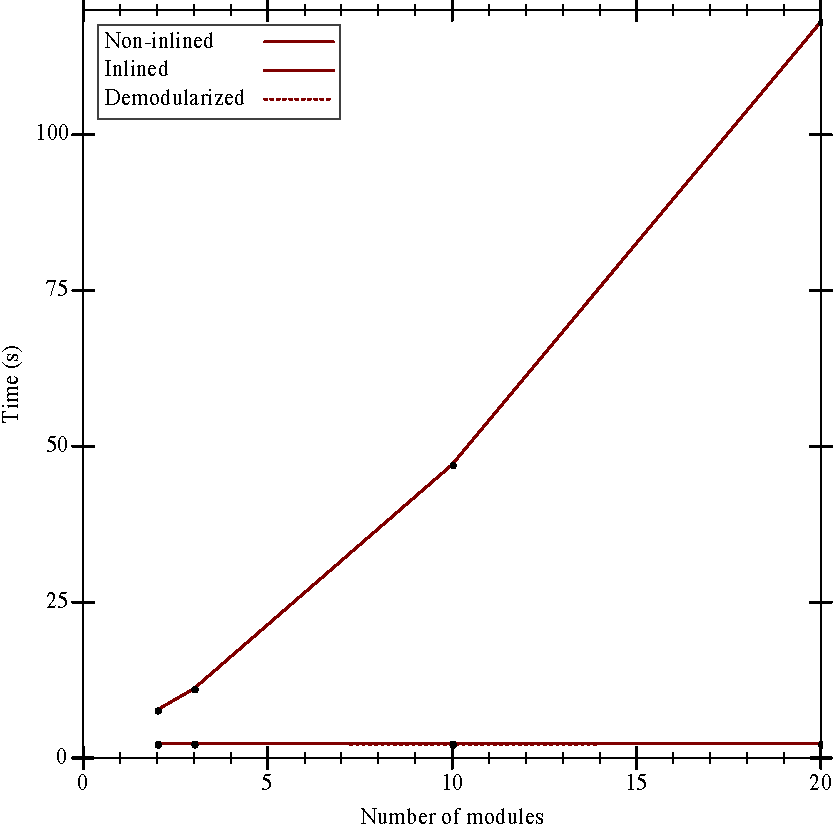
\includegraphics{figures/micro-results}
\caption{Results from micro benchmarks}
\label{fig:micro-results}
\end{figure}
Without inlining, the micro benchmarks increase in a linear fashion with an increase in the number of modules.
With inlining, the micro benchmarks stay at a constant speed.
With demodularization, the micro benchmarks also stay at a constant speed, with a slightly better speed than inlining.
Both inlining and demodularization result in similar final bytecode, where the only difference is how many times the loop is unrolled.
The cross-module inlining algorithm is more complicated than the demodularization algorithm, so there are cases where inlining would fail and demodularization would not. 
The inlining algorithm creates annotations on the bytecode of functions, which it must track and update.
If a function is too large, the algorithm will not inline it (even if it is only used once). 
Demodularization does not have these limitations because it every function in the program is available to the optimizer as if it were a local function. 
Therefore, it would be possible to create a benchmark that differentiates between cross-module inlining and demodularization by creating functions that are too large to inline, but would still be optimized in the demodularized program.

\section{Macro Benchmarks}
For macro benchmarks we selected programs that would terminate deterministically and that used multiple modules.
One of the programs we tested was a program that uses the Racket XML library to read large XML files.
The program can be found in Appendix~\ref{chap:benchmarks}.
For test data, we used astronomical data from NASA~\cite{nasa}. 
The second program we tested is a benchmark for the Redex tool.
Redex is a library that allows users to build and test semantic models.
We also tested uses of the math and plot libraries, which are written in a modular way. 
Figure~\ref{fig:macro-results} shows the results of running demodularization on larger programs.
\begin{figure}
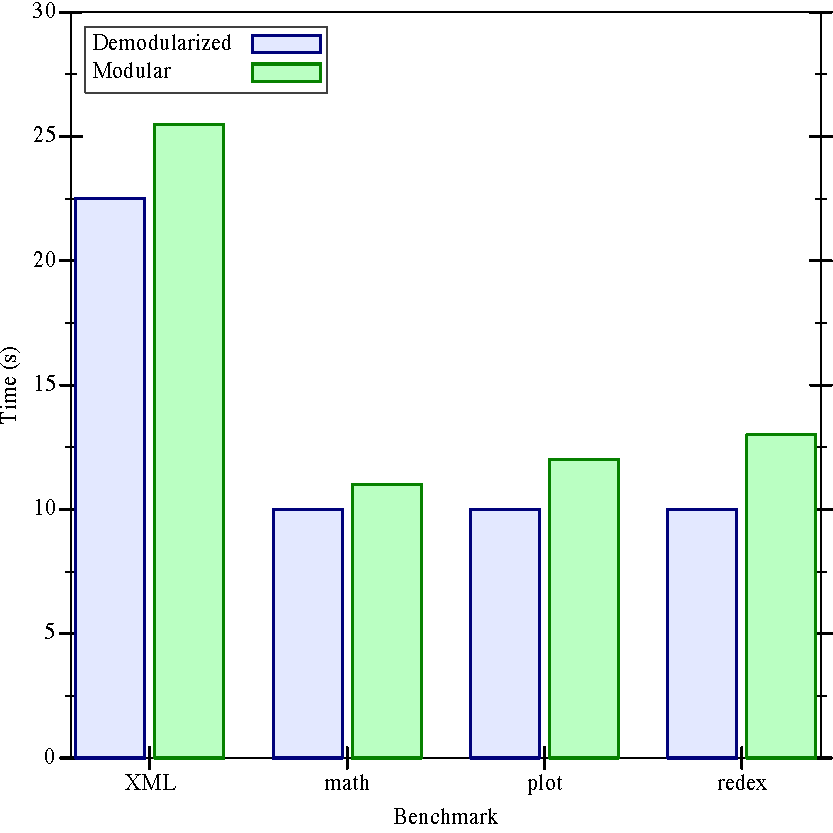
\includegraphics[width=.8\textwidth]{figures/macro-results}
\caption{Results from macro benchmarks}
\label{fig:macro-results}
\end{figure}

\section{Dead Code Elimination}
As an experiment, we implemented an unsound dead code elimination algorithm for demodularized programs.
It identifies all uses of toplevel definitions in the body of the demodularized program and eliminates all other toplevels.
The reason it is unsound is because although some toplevels may not be referenced directly in the program, they may be needed for side-effects that they have.
These side-effects may include setting up global objects or tables that will be referenced by the program, or I/O operations.
In order to make the dead code elimination algorithm sound, we would need to identify primitives that can have side-effects and include any toplevels that use those primitives.
This would be possible to do with some engineering effort, but it is beyond the scope of this work. 
The experiment gives a lower-bound on the performance of this optimization, so it is a useful result.
Figure~\ref{fig:dead-code} shows how much smaller programs become after running the dead code elimination algorithm on them.
\begin{figure}
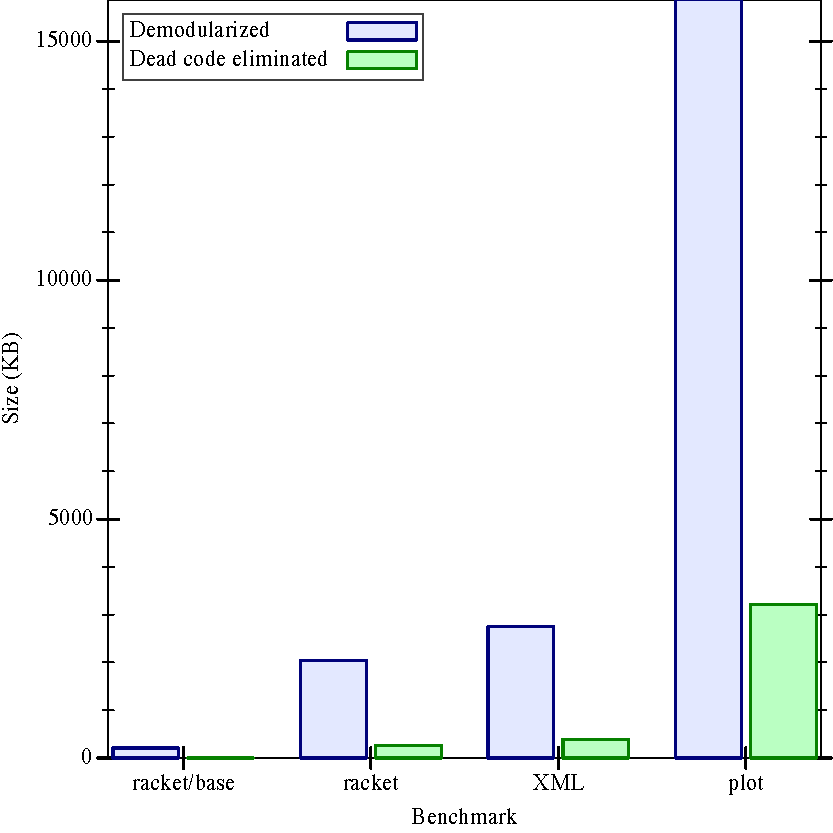
\includegraphics[width=.8\textwidth]{figures/gc-results}
\caption{Dead code elimination results}
\label{fig:dead-code}
\end{figure}
When dead code is eliminated it opens up opportunities for other optimizations because the code is smaller.
It opens up opportunities for inlining functions that are used a small number of times or determining if the values of arguments are the same.
Also, smaller code size can be a benefit by itself in space constrained or networked systems.

\section{Further Optimizations}

Having access to the whole-program at once enables optmizations that currently are not implemented by the Racket optimizer.
For example, any optimizations that rely on Control-Flow Analysis (CFA) \cite{cfa} require access to the whole program.
These include type test eliminations and inlining inside function definitions based on arguments.
Demodularization enables these sorts of optmiziations to be performed on modular programs.

Demodularization is a simple solution to the optimization problems that arise from modular programming. 
Even just using existing optimizations that were not implemented with whole programs in mind, we see some benefits in performance. 
When new optimizations are developed that take advantage of whole programs, we should see even bigger improvements in performance.

\chapter{Related Work}
\label{chap:related-work}
Prior work on whole-program optimization has come in two flavors, depending on how much access to the source code the optimizer has. The first approach assumes full access to the source code and is based on inlining. The second approach only has access to compiled modules and is based on combining modules.

The first approach is based on selectively inlining code across module boundaries because it has full access to the source code of the program \cite{258960,Chambers96whole-programoptimization}. Most of the focus of this approach is finding appropriate heuristics to inline certain functions without ballooning the size of the program and making sure the program still produces the same results. Resulting programs are not completely demodularized; they still have some calls to other modules. Specifically, Chambers et al. \cite{Chambers96whole-programoptimization} show how this approach applies to object-oriented languages like C++ and Java, where they are able to exploit properties of the class systems to choose what to inline. Blume and Appel \cite{258960} showed how to deal with inlining in the presence of higher order functions, to make sure the semantics of the program didn't change due to inlining. Their approach led to performance increases of around 8\%.

The second approach is taking already compiled modules, combining them into a single module, and optimizing the single module at link time \cite{sutter,727617}. Most of the work done with this approach optimized at the assembly code level, but because they were able to view the whole program, the performance increases were still valuable. 
The link-time optimization system by Sutter et al. \cite{sutter} achieves a 19\% speedup on C programs.
One of the reasons for starting with compiled modules is so that programs using multiple languages can be optimized in a common language, like the work done by Debray et al. \cite{727617} to combine a program written in both Scheme and Fortran. The main problem with this approach is that the common language has less information for optimization than the source code had. 
These approaches are similar to demodularization, but they operate at a lower level and work on languages without phased module systems.


\chapter{Conclusion}
\label{chap:conclusion}

Demodularization is a useful optimization for deploying modular programs. 
A programmer can write a modular program and get the benefits of separate compilation while devloping the program, and then get additional speedups by running the demodularizer on the completed program.
Demodularization also enables new optimizations that are not feasible to implement for modular programs.
Without module boundaries, inter-procedural analysis is much easier and worthwhile.
Also, dead code elmination works much better because the whole program is visible, while in a modular program, only dead code that is private to the module can be eliminated.

In the future, we would like to implement an aggressive dead code elimination algorithm for Racket.
% TODO: what does it mean to ignore side effects, why does it matter?
We implemented a naive one that does not respect side effects, but shows the potential gains from this optimization; it is able to shrink Racket binaries down from about 2MB to about 100KB\@.
This promising result implies that other low-hanging optimizations should be possible on demodularized programs that can increase performance.



\bibliographystyle{plain}
\bibliography{bib}

\end{document}
